\documentclass{article}
\usepackage[spanish]{babel}
\usepackage{graphicx}
\usepackage{listings}
\setlength{\parindent}{0pt}
\setlength{\parskip}{3mm}
\usepackage[numbers]{natbib}
\usepackage{color}
\definecolor{dkgreen}{rgb}{0,0.6,0}
\definecolor{gray}{rgb}{0.5,0.5,0.5}
\definecolor{mauve}{rgb}{0.58,0,0.82}

\usepackage{geometry}


\addtolength{\topmargin}{-.70in}
\addtolength{\textheight}{1in}

\lstset{ 
  backgroundcolor=\color{white},   % choose the background color; you must add \usepackage{color} or \usepackage{xcolor}; should come as last argument
  basicstyle=\footnotesize,        % the size of the fonts that are used for the code
  breakatwhitespace=false,         % sets if automatic breaks should only happen at whitespace
  breaklines=true,                 % sets automatic line breaking
  captionpos=b,                    % sets the caption-position to bottom
  commentstyle=\color{dkgreen},    % comment style
  deletekeywords={...},            % if you want to delete keywords from the given language
  escapeinside={\%}{)},          % if you want to add LaTeX within your code
  extendedchars=true,              % lets you use non-ASCII characters; for 8-bits encodings only, does not work with UTF-8
  firstnumber=1,                % start line enumeration with line 1000
  frame=single,	                   % adds a frame around the code
  keepspaces=true,                 % keeps spaces in text, useful for keeping indentation of code (possibly needs columns=flexible)
  keywordstyle=\color{blue},       % keyword style
  language=Octave,                 % the language of the code
  morekeywords={*,...},            % if you want to add more keywords to the set
  numbers=left,                    % where to put the line-numbers; possible values are (none, left, right)
  numbersep=5pt,                   % how far the line-numbers are from the code
  numberstyle=\tiny\color{gray}, % the style that is used for the line-numbers
  rulecolor=\color{black},         % if not set, the frame-color may be changed on line-breaks within not-black text (e.g. comments (green here))
  showspaces=false,                % show spaces everywhere adding particular underscores; it overrides 'showstringspaces'
  showstringspaces=false,          % underline spaces within strings only
  showtabs=false,                  % show tabs within strings adding particular underscores
  stepnumber=1,                    % the step between two line-numbers. If it's 1, each line will be numbered
  stringstyle=\color{mauve},     % string literal style
  tabsize=2,	                   % sets default tabsize to 2 spaces
  title=\lstname                  % show the filename of files included with \lstinputlisting; also try caption instead of title
}
\title{
Tarea 2
}
\author{5280}
\date{\today}

\begin{document}

\maketitle


\section*{Introducción}

La teoría de grafos tiene aplicación en diversas áreas, debido a que las redes aparecen prácticamente en todas las actividades de nuestra vida diaria: sistemas de comunicaciones, sistemas hidráulicos, circuitos eléctricos y electrónicos, sistemas mecánicos, redes sociales, entre otros. 

Como constata Ravindra \cite{ahuja2017network}, las redes físicas son quizás las más comunes y mejor identificables. Los sistemas de transporte, cualquiera que sea el medio suelen modelarse en sistemas de distribución  y decisiones logísticas complejos, siendo el Problema de transporte un ejemplo típico de investigación de operaciones. 

Otro ejemplo representativo de uso de grafos son los algoritmos de búsqueda web de Google. Estos se basan en el gráfico WWW, que contiene todas las páginas web como vértices y los  hipervínculos como bordes \cite{chung2010graph}.

La teoría de los grafos también ha sido usada en química, debido a la posibilidad de representar los modelos estructurales mediante diagramas. En un grafo molecular, los vértices representan a los átomos y los lados a los enlaces químicos que conectan ciertas parejas de átomos \cite{amador}.

Para acomodar los grafos, de manera que su forma refleje lo que se desea, se han desarrollo varios layouts: algoritmos que devuelven una lista de posiciones para los nodos, según  parámetros definidos.

Entre los layouts más conocidos se destacan:
\begin{itemize}

\item Bipartite layout
\item Circular layout
\item Kamada kawai layout
\item Random layout
\item Rescale layout
\item Shell layout
\item Spring layout
\item Spectral layout
\end{itemize}

\section{Grafo simple no dirigido acíclico}

La mayoría de los esquemas de líneas de autobuses, tranvías o trenes del transporte público pueden ser representados por grafos simples no dirigidos acíclicos.

En la figura  \ref{Figura 1} se muestra una sección de ochos estaciones de la Línea 2 del Metro de Monterrey, donde las estaciones son los nodos y el tramo de línea entre ellos, los vértices. 

Para posicionar los nodos de este grafo se empleó el spring layout. Se obtuvieron resultados igualmente satisfactorios empleando otros layouts.

\begin{figure}
\begin{center}
  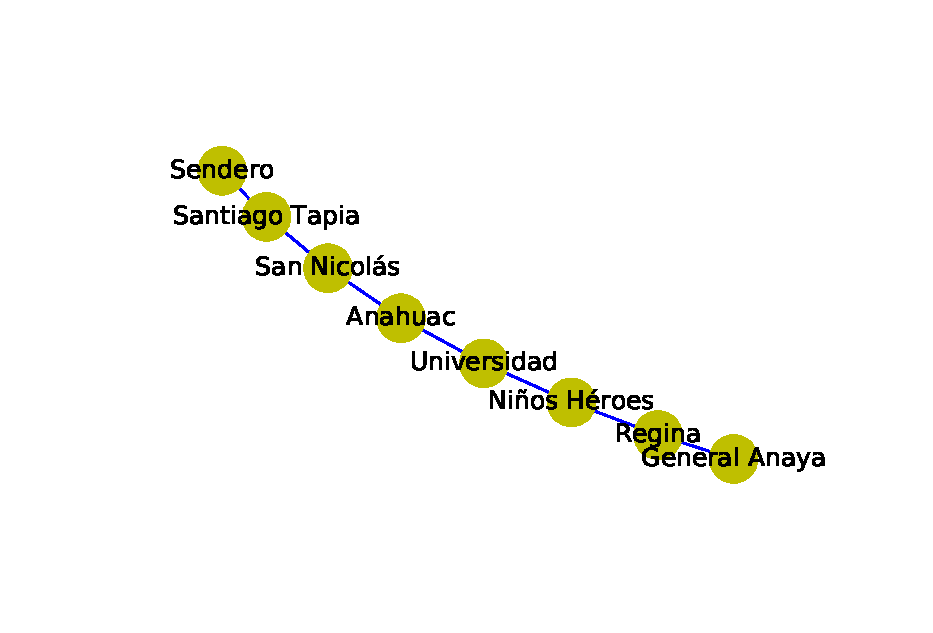
\includegraphics[width=.7\columnwidth]{fig1.eps}
   \end{center}
  \caption{Representación con un grafo de ocho estaciones de la Línea 2 del Metro de Monterrey.}
  \label{Figura 1}
 
\end{figure}

\lstinputlisting[language=Python]{Ej1.py}

\section{Grafo simple no dirigido cíclico}

Este tipo de grafos es adecuado para representar relaciones comerciales entre empresas al igual que relaciones de parentezco, amistad o romance entre personas.
En la figura \ref{Figura 2} se muestra un grafo que representa las relaciones de amistad en un grupo de diez personas. Los vértices son las personas y las aristas, las personas que tienen una relación de amistad.

Para posicionar este grafo se usó el Fruchterman-Reingold layout. Este fue diseñado para dibujar gráficos no dirigidos, con el objetivo de distribuir los vértices uniformemente en el marco, haciendo que las longitudes de los bordes sean uniformes y reflejando la simetría \cite{fruchterman1991graph}.
 
\begin{figure}
 \begin{center}
  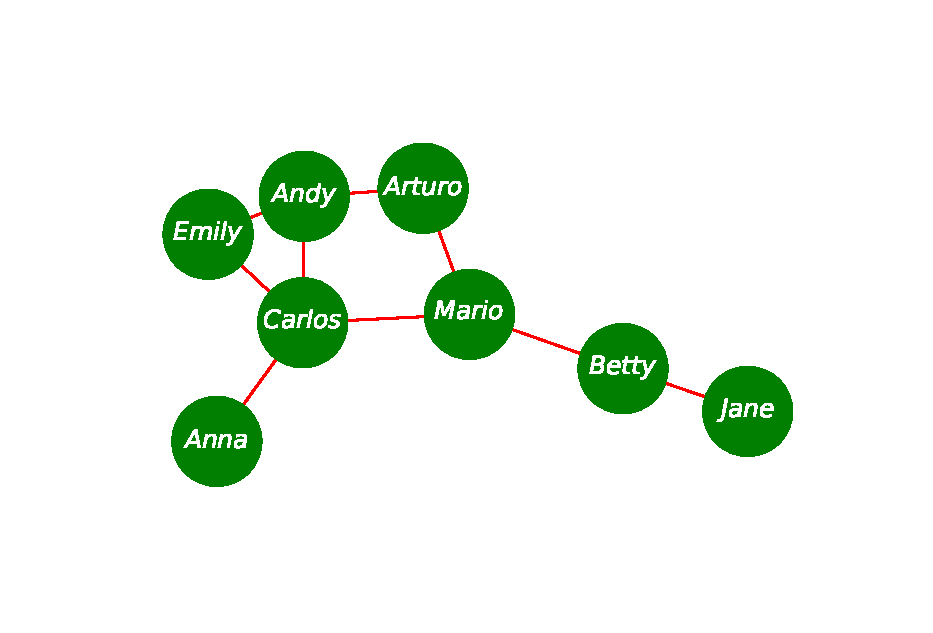
\includegraphics[width=.6\columnwidth]{fig2.eps}
   \end{center}
  \caption{Relaciones de amistad en un grupo de personas.}
  \label{Figura 2}
\end{figure}

\lstinputlisting[language=Python]{Ej2.py}

\section{Grafo simple no dirigido reflexivo}

Un criador de perros posee seis razas diferentes de estos animales. Con un grafo de este tipo puede representar de cuales de estos animales ha obtenido crías, siendo los vértices las razas de perro y las aristas la unión entre razas que han tenido crías.

En la figura \ref{Figura 3} se puede observar que todas las razas excepto la Beagle, que es recién adquirida y aún no se ha reproducidos, han tenido crías con su misma raza (vértices en rojo). También se observa que han habido cruzamientos entre bóxer y bulldog y entre pitbull y rottweiler.

Para posicionar este grafo se usó el Kamada-Kawai layout, diseñado para dibujar grafos ponderados no dirigidos \cite{kamada1989algorithm}. Los layouts circular y shell mostraron también resultados similares.


\begin{figure}
  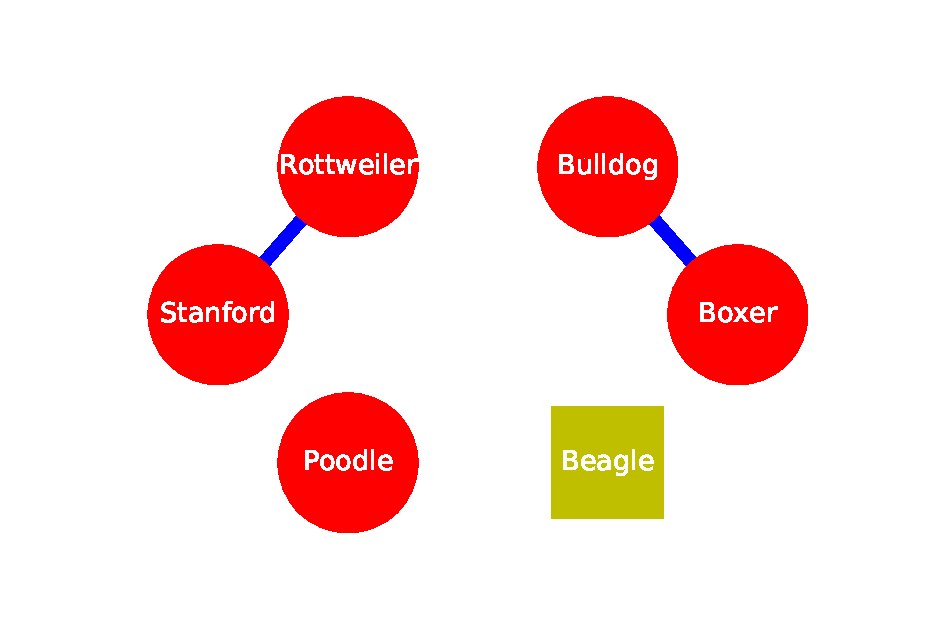
\includegraphics[width=.8\columnwidth]{fig3.eps}
  \caption{Estado de cría de razas de perro}
  \label{Figura 3}
\end{figure}

\lstinputlisting[language=Python]{Ej3.py}

\section{Grafo simple dirigido acíclico}

La cadena de propagación de las ITS (Infecciones de Transmisión Sexual) para las cuales no se conoce cura o las que solo afectan al individuo una vez en la vida, pueden representarse mediante grafos simples dirigidos acíclicos. En este caso cada sujeto es un vértice y la dirección de transmisión de la enfermedad es representada en la arista. Desde la enfermedad se propaga desde la persona portadora hacia el sujeto sano que posteriormente se convierte en portador y contagia a otros sujetos sanos.

De los layouts empleados para posicionar los elementos de la figura \ref{Figura 4} el Fruchterman-Reingold fue el más adecuado.

\begin{figure}
  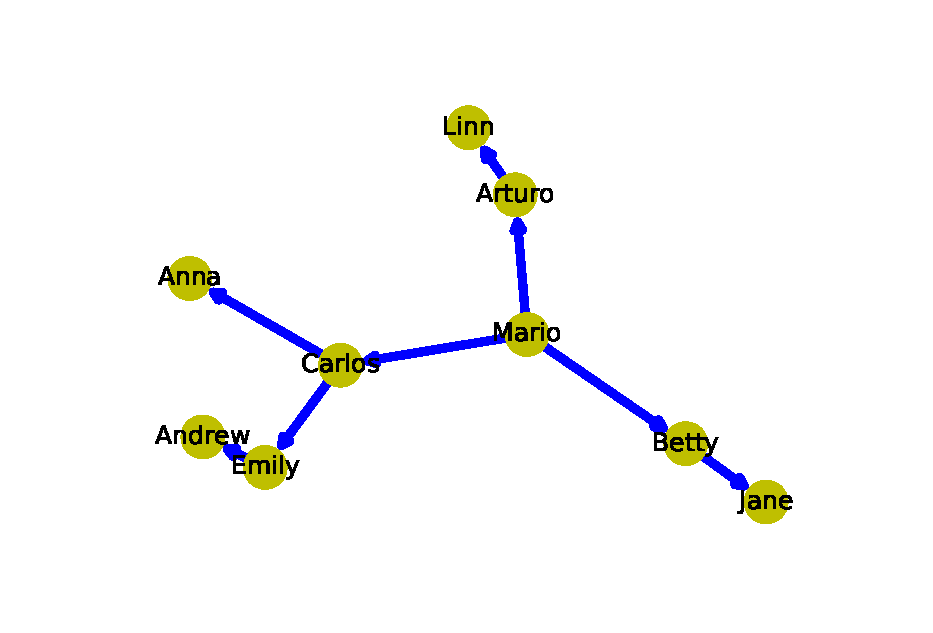
\includegraphics[width=.8\columnwidth]{fig4.eps}
  \caption{Representación de la transmisión de una ITS en un grupo de personas.}
  \label{Figura 4}
\end{figure}
\newpage
\lstinputlisting[language=Python]{Ej4.py}

\section{Grafo simple dirigido cíclico}

En ciudades con carreteras estrechas como Santiago de Cuba, en diferentes sectores, las carreteras son de un solo sentido y se representan con grafos de este tipo. Las aristas representan las calles y los vértices son las intersecciones entre al menos dos aristas.

Luego de probar varios layouts, el spectral fue el que arrojó el resultado deseado para dibujar la figura \ref{Figura 5}.

\begin{figure}
  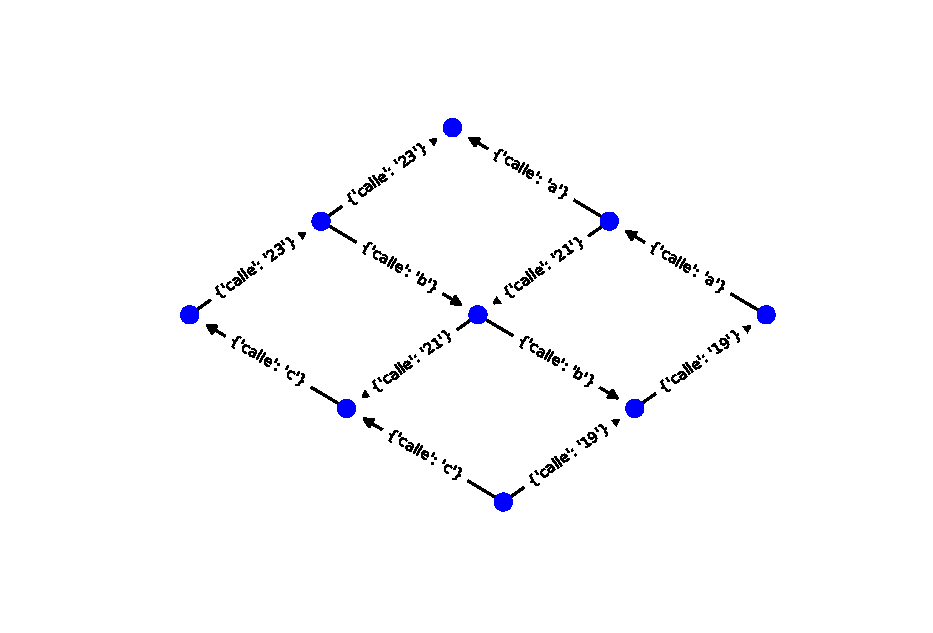
\includegraphics[width=.8\columnwidth]{fig5.eps}
  \caption{Carreteras de sentido único en Santiago de Cuba.}
  \label{Figura 5}
\end{figure}

\lstinputlisting[language=Python]{Ej5.py}


\section{Grafo simple dirigido reflexivo}

Un grafo en el que cada vértice es una empresa de servicios y las aristas, la unión con cada una de las otras empresas a las que le presta servicios, puede representarse mediante un grafo dirigido reflexivo, pues algunas de estas empresas se brindan servicio a ellas mismas. 

Un sitio web pequeño, en el cual se accede a todas sus páginas a través de un menú estático también se puede representar con este tipo de grafo. 

Otro ejemplo está dado por la representación de un grupo de personas conectadas a una red social y los perfiles de otras personas que tengan abiertos en el navegador en ese momento. Cada una de esas persona también pudiesen estar mirando su propio
perfil. En el grafo de la figura \ref{Figura 6} los vértices son las personas y las aristas indican el perfil de qué personas tiene cada uno abierto en el navegador. Puede apreciarse en color rojo que Mayra y Andrew tienen abiertos sus propios perfiles.

Para obtener la forma deseada del grafo dieron resultados similares el circular layout y el shell.


\begin{figure}
\begin{center}
  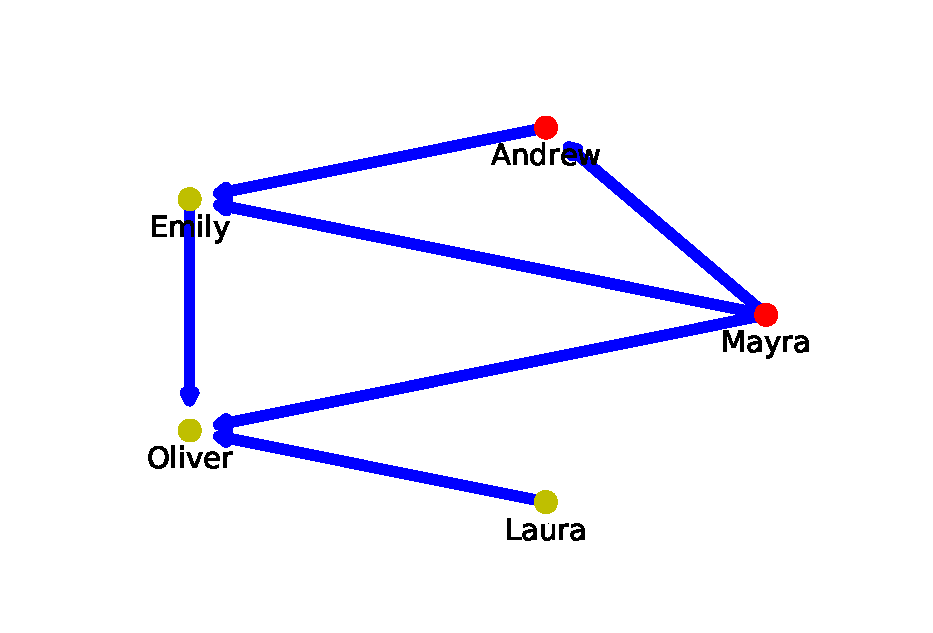
\includegraphics[width=.6\columnwidth]{fig6.eps}
  \end{center}
  \caption{Representación de personas mirando perfiles en redes sociales.}
  \label{Figura 6}
\end{figure}

\lstinputlisting[language=Python]{Ej6.py}


\section{Multigrafo no dirigido acíclico}

La ruta entre Santiago de Cuba y Holguín puede representarse  como un multigrafo no dirigido cíclico. En un pueblo llamado Caballería la carretera principal se bifurca, pudiendo continuar por la ruta principal hasta Banes, o por el camino alternativo de Caballería, que, aunque es más largo, puede recorrerse en menor tiempo a causa del poco tránsito.

En la figura \ref{Figura 7} los vértices representan las cabeceras municipales, que están simplemente enumeradas por no ser de interés para el ejemplo mencionado. Para la visualización se empleó el layout Kamada-Kawai.

\begin{figure}
  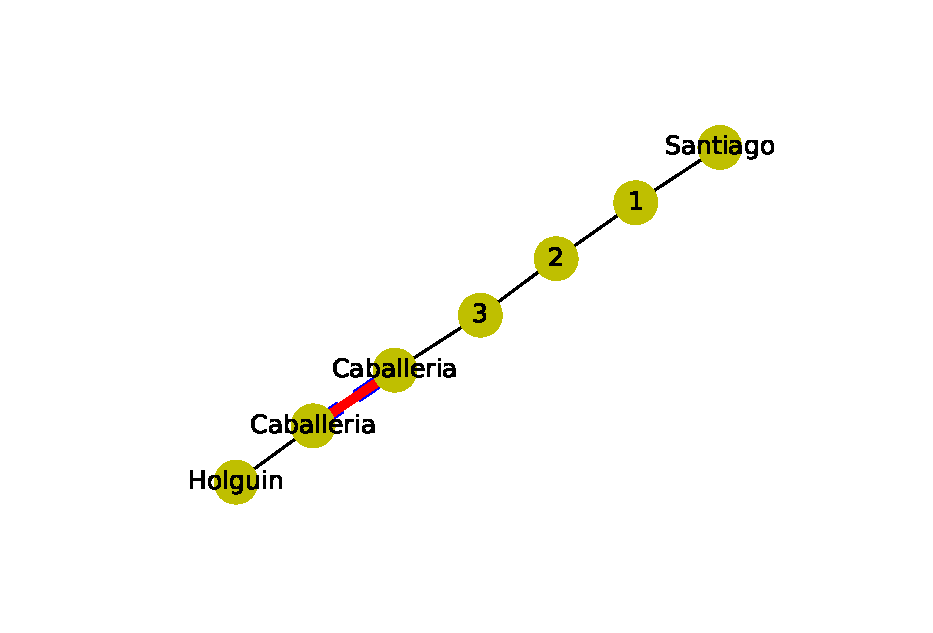
\includegraphics[width=.8\columnwidth]{fig7.eps}
  \caption{Posible ruta entre Santiago de Cuba y Holguín}
  \label{Figura 7}
\end{figure}

\lstinputlisting[language=Python]{Ej7.py}


\section{Multigrafo no dirigido cíclico}

En la presa El cacao, ubicada en el Municipio Cotorro, Ciudad de La Habana, se realizó un proyecto para favorecer la agricultura. Al rededor de la presa se construyeron una serie de canales para mantener el suelo húmedo durante todo el año.
Este sistema puede ser representado mediante el grafo de la figura \ref{Figura 8}, el cual los vértices representan la unión entre uno o más canales y las aristas, cada uno de los canales. El layout Kamada-Kawai fue el que mejores resultados de visualización arrojó.

\begin{figure}
  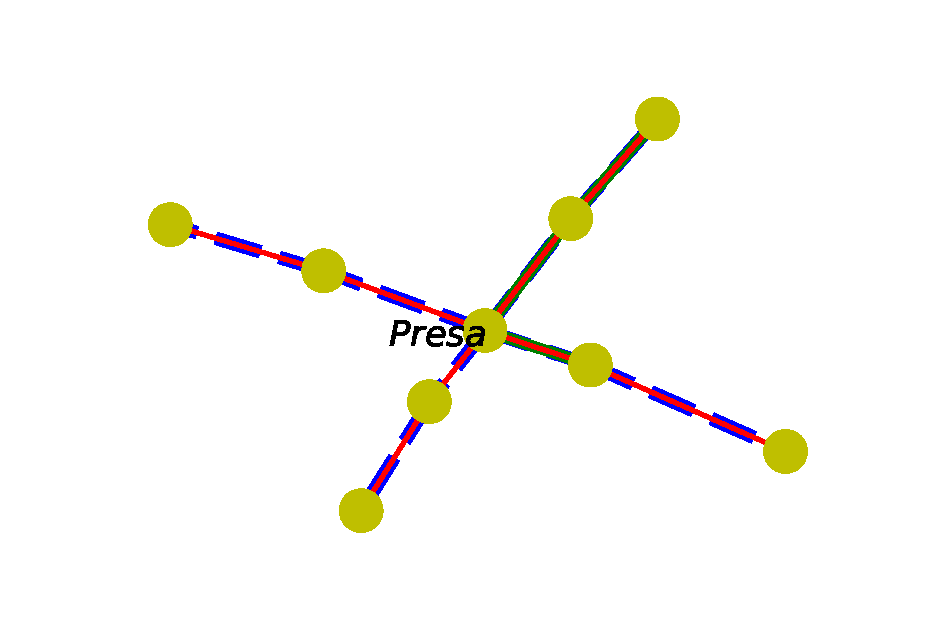
\includegraphics[width=.8\columnwidth]{fig8.eps}
  \caption{Canales para irrigación del suelo creados en la presa El cacao.}
  \label{Figura 8}
\end{figure}
\newpage
\lstinputlisting[language=Python]{Ej8.py}


\section{Multigrafo no dirigido reflexivo}

En la Universidad de Oriente se quiere realizar un concurso de habilidades entre las carreras de Ingeniería en Electrónica, Ingeniería en Automática, Licenciatura en Física, Ingeniería en Informática y Licenciatura en Matemática-Cibernética. Las habilidades a evaluar serán matemática y programación. 

La figura \ref{Figura 9} muestra como está organizado el concurso. Cada vértice representa a los estudiantes que estudian una de las carreras y las aristas, con qué estudiantes pueden participar en cada habilidad. Todos los vértices son de color rojo porque todos los estudiantes pueden competir con estudiantes de su misma carrera.

Los vértices rojos unen a los que pueden concursar en entre sí en matemáticas y los azules, los que pueden concursar en programación.

Para la visualización se empleó el layout circular.

\begin{figure}
  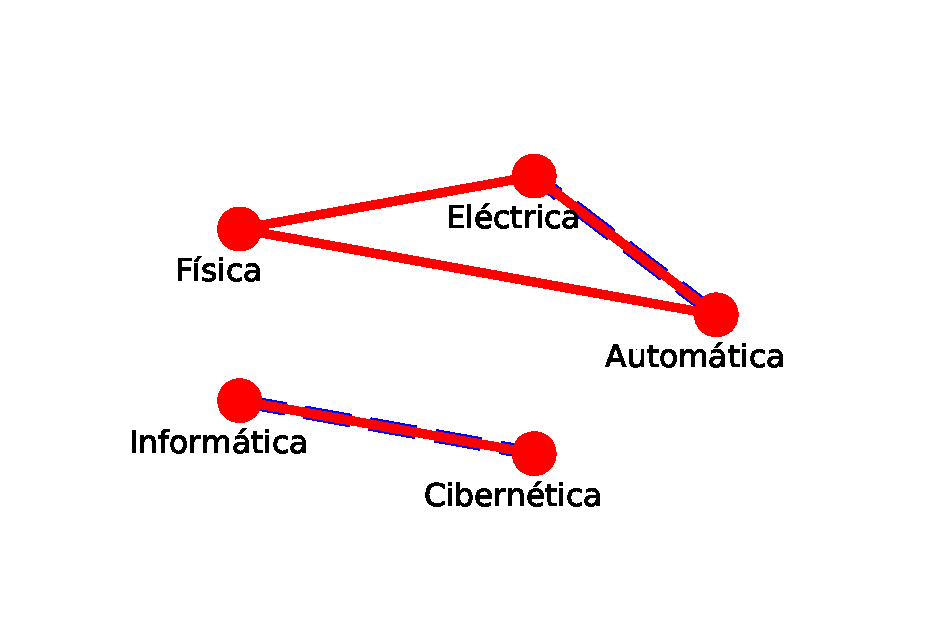
\includegraphics[width=.8\columnwidth]{fig9.eps}
  \caption{Concurso de habilidades.}
  \label{Figura 9}
\end{figure}

\lstinputlisting[language=Python]{Ej9.py}


\section{Multigrafo dirigido acíclico}

Estos grafos pueden utilizarse para representar la cuenca hidrográfica de un río en su flujo hacia el mar. En la figura \ref{Figura 10}los vértices representan los puntos en los que al menos dos ramificaciones del delta confluyen o se separan. Para que el grafo tiviese exactamente la forma deseada, se insertaron las coordenadas de los nodos de manera manual.

\begin{figure}
  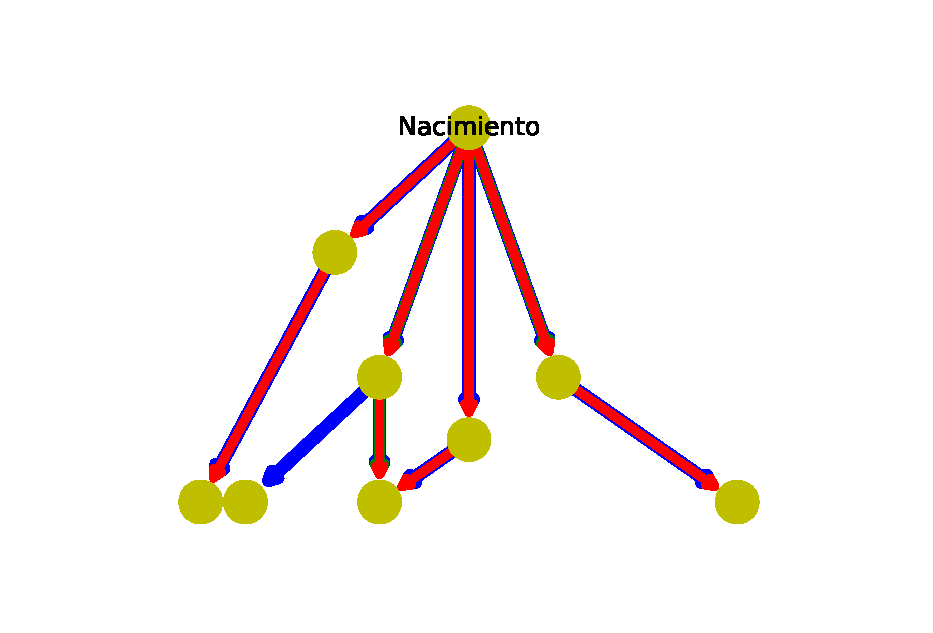
\includegraphics[width=.8\columnwidth]{fig10.eps}
  \caption{Representación del delta de un río en su transcurso hacia el mar.}
  \label{Figura 10}
\end{figure}

\lstinputlisting[language=Python]{Ej10.py}


\section{Multigrafo dirigido cíclico}

Este tipo de grafo es especialmente útil para representar viajes por lugares a los que se puede llegar mediante diferentes vías, regresando luego al punto de origen. Un ejemplo concreto de esto sería un recorrido vacacional por varias ciudades. Partiendo de la ciudad A, hay tres posibles vías  para llegar a la ciudad B, en bus, en auto de alquiler o en tren, cada uno de estos medios de transporte representaría una arista diferente para unir los vértices. Así sucesivamente, se tienen en cuenta las posibles vías de transporte hacia las distintas ciudades hasta completar el recorrido y regresar a casa. 

Para posicionar los vértices en la figura \ref{Figura 11} se empleó el layout shell, aunque el circular también ofrece buenos resultados en este tipo de grafos.


\begin{figure}
\begin{center}
  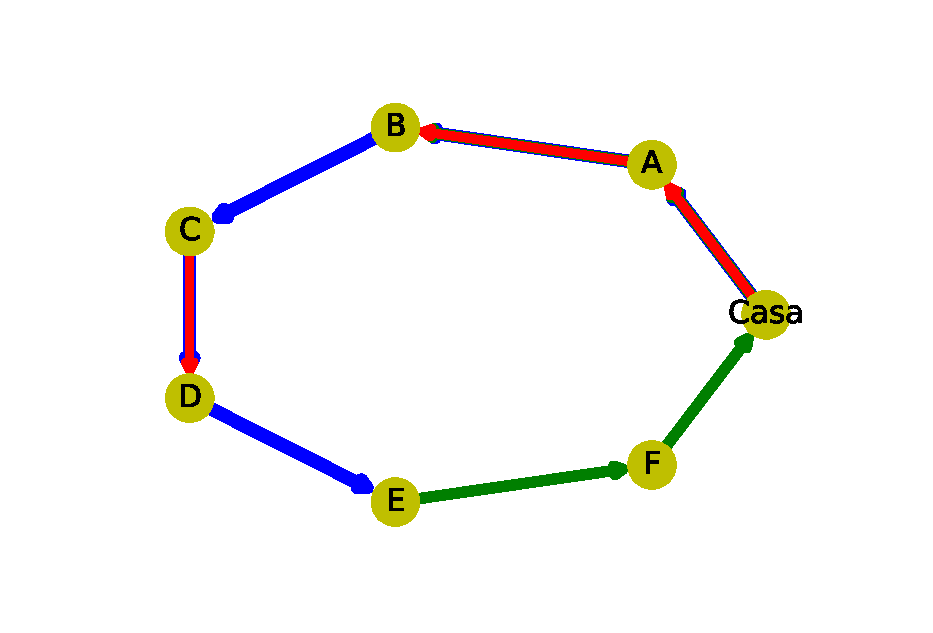
\includegraphics[width=.6\columnwidth]{fig11.eps}
  \caption{Representación de las posibles maneras de elegir la ruta de un circuito vacacional.}
  \end{center}
  \label{Figura 11}
\end{figure}

\lstinputlisting[language=Python]{Ej11.py}


\section{Multigrafo dirigido reflexivo}

González-Cervantes \cite{gonzalez2016potencial} empleó teoría de grafos para representar el potencial eléctrico en el corazón, demostrando que se pueden incorporar las leyes fisiológicas involucradas. Cada uno de los vértices representa uno de los puntos principales que generan los impulsos eléctricos y que llevan la electricidad a cada parte del corazón, las aristas describen el valor máximo de voltaje y su
duración en tiempo que descarga cada vértice. Además, puede proporcionar información con respecto al potencial eléctrico por zonas para una mejor localización.
En la figura \ref{Figura 12} se muestra la representación con grafos del intervalo PR. Debido a que se siguió la forma del corazón para dibujar el grafo, las coordenadas de los vértices fueron ingresadas manualmente.


\begin{figure}
  \centering 
  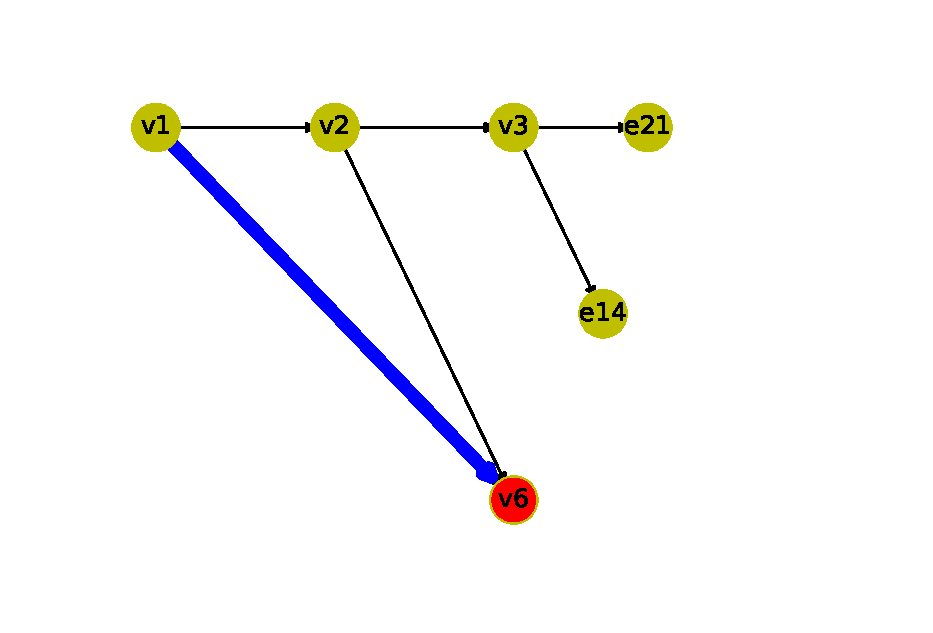
\includegraphics[width=.8\columnwidth]{fig12.eps}
  \caption{Representación con grafos del intervalo PR.}
  \label{Figura 12}
\end{figure}

\lstinputlisting[language=Python]{Ej12.py}



%-------------------------------------------------------------------------------
% References
%-------------------------------------------------------------------------------
\newpage
\bibliography{Tarea2}
\bibliographystyle{plain}



\end{document}
